\documentclass{article}

\usepackage{graphicx}
\usepackage{amssymb}
\usepackage{amsmath}
\usepackage{cancel}

\newcommand\linvel{\mathbf{v}}
\newcommand\trans{\mathbf{t}}
\newcommand\conf{\mathbf{q}}
\newcommand\reals{\mathbb{R}}

\title{Computation of the exact inverse kinematics solution of a 6D robotic arm}
\author{Florent Lamiraux - CNRS}

\begin{document}
\maketitle

\begin{figure}
  \begin{center}
    \def\svgwidth {.6\linewidth}
    \graphicspath{{./figures/}}
    \input{figures/kinematic-chain.pdf_tex}
  \end{center}
  \caption{Input (blue) and output (red) variables of the explicit constraint that computes the robot arm configuration with respect to the handle pose.}
  \label{fig:kinematic-chain}
\end{figure}

\section{Introduction}

This document explains how to implement exact inverse kinematics of a Stäubli robotic arm as an
explicit constraint in Humanoid Path Planner software. Notation and definitions are the same as
in~\cite{lamiraux:hal-02995125}.

\section{Notation and Definitions}

The constraint is defined as a 6 dimensional \textit{grasp} constraint between a \textit{gripper} and a
\textit{handle}. The \textit{gripper} is attached to the robotic arm end-effector (\texttt{joint1}) and the \textit{handle} is attached to \texttt{joint2} on the composite kinematic chain. \texttt{root} is the joint that holds the robot arm or the global frame (\texttt{"universe"} in \texttt{pinocchio} software).

We denote by
\begin{itemize}
\item $\conf_{in}$ the input variables of the explicit constraint,
\item $\conf_{out}$ the output variables of the explicit constraint,
\item $^0M_1$ the pose of \texttt{joint1} in the world frame,
\item $^0M_2$ the pose of \texttt{joint2} in the world frame,
\item $^0M_r$ the pose of \texttt{root} in the world frame,
\item $^2M_h$ the pose of the handle in \texttt{joint2} frame,
\item $^1M_g$ the pose of the gripper in \texttt{joint1} frame,
\item $^rM_b$ the pose of the robot arm origin (\texttt{base\_link} in URDF
  description) in the \texttt{root} frame.
\end{itemize}

\section{Inverse kinematics}

Exact inverse kinematics computes the 6 joint values of the robotic arm with
respect to the input configuration variables:
\begin{equation}\label{eq:inverse-kinematics}
  \conf_{out} = f(\conf_{in})
\end{equation}
Note that the input variables include a extra degree of freedom that is interpreted as an integer to select among the various solutions of the inverse kinematics.

\begin{figure}[h]
  \centering
  \graphicspath{{./figures/}}
  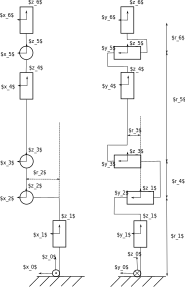
\includegraphics[width=0.5\textwidth]{staubli-TX90-schematic.pdf}
\end{figure}
For the Staubli TX90, we have the following cotation in meters:
\begin{align*}
  r1&=0.478\\
  r2&=0.050\\
  r3&=0.05\\
  r4&=0.425\\
  r5&=0.425\\
  r6&=0.1\\
\end{align*}
We are going to use the following schematic to determinate each transformation matrix for each frame.
We denote by:
\begin{itemize}
\item $T_{i-1,i}$ the homogeneous transformation matrix from frame $i-1$ to frame $i$,\\
\item $T_{0,1}$ the transformation matrix from base link to the first joint frame,\\
\item $T_{5,6}$ the transformation matrix from joint 5 frame to the gripper frame,\\
\end{itemize}
Homogeneous transformation matrix  $T_{i-1,i}$  from frame $i-1$  to frame $i$  :

\[
\begin{array}{cc}
T_{0,1} =
\begin{bmatrix}
  \cos(q_1) & -\sin(q_1) & 0 & 0 \\
  \sin(q_1) & \cos(q_1) & 0 & 0 \\
  0 & 0 & 1 & r_1 \\
  0 & 0 & 0 & 1 \\

\end{bmatrix}

&

T_{1,2} =
\begin{bmatrix}
  \cos(q_2) & 0 & \sin(q_2) & r_2 \\
  0 & 1 & 0 & 0 \\
  -\sin(q_2) & 0 & \cos(q_2) & 0 \\
  0 & 0 & 0 & 1 \\

\end{bmatrix}
\end{array}
\]

\[
\begin{array}{cc}
T_{2,3} =
\begin{bmatrix}
  \cos(q_3) & 0 & \sin(q_3) & 0 \\
  0 & 1 & 0 & r_3 \\
  -\sin(q_3) & 0 & \cos(q_3) & r_4 \\
  0 & 0 & 0 & 1 \\

\end{bmatrix}
&
T_{3,4} =
\begin{bmatrix}
  \cos(q_4) & -\sin(q_4) & 0 & 0 \\
  \sin(q_4) & \cos(q_4) & 0 & 0 \\
  0 & 0 & 1 & 0 \\
  0 & 0 & 0 & 1 \\

\end{bmatrix}
\end{array}
\]
\[
\begin{array}{cc}
T_{4,5} =
\begin{bmatrix}
  \cos(q_5) & 0 & \sin(q_5) & 0 \\
  0 & 1 & 0 & 0 \\
  -\sin(q_5) & 0 & \cos(q_5) & r_5 \\
  0 & 0 & 0 & 1 \\

\end{bmatrix}

&

T_{5,6} =
\begin{bmatrix}
  \cos(q_6) & -\sin(q_6) & 0 & 0 \\
  \sin(q_6) & \cos(q_6) & 0 & 0\\
  0 & 0 & 1 & r_6\\
  0 & 0 & 0 & 1\\

\end{bmatrix}
\end{array}
\]


Calculation of  $T_{0,5}$ and $T_{3,6}$ to determinate each configuration expressions, we only use the translation vector to determinate the concurant point. We assume that $sin(q_i)=s_i$  for each i between 1 and 6. \\
\begin{align*}
T_{0,3} = T_{0,1} T_{1,2} T_{2,3} T_{3,4} T_{4,5} =
\begin{bmatrix}
  X & X & X &r_5c_1s_{2+3}-r_3s_1+r_4c_1s_2+c_1r_2\\
  X & X & X & r_5s_1s_{2+3}+r_3c_1+r_4s_1s_2+r_2s_1 \\
  X & X & X & r_5c_{2+3}+r_4c_2+r_1 \\
  0 & 0 & 0 & 1 \\
\end{bmatrix}
\end{align*}

\[
T_{3,6} = T_{3,4} T_{4,5} T_{5,6}= \\
\begin{bmatrix}
  c_4c_5c_6+s_4s_6 & -c_4c_5s_6-s_4c_6 & c_4s_5 & r_6c_4s_5 \\
  s_4c_5c_6-c_4s_6 & -s_4c_5s_6+c_4c_6 & s_4s_5 & r_6s_4s_5 \\
  -s_5c_6 & s_5s_6 & c_5 & r_6c_5 + r_5 \\
  0 & 0 & 0 & 1 \\
\end{bmatrix}
\]

In order to know the configuration for the position of the concourant point, we need to use the translation vector in $T_{0,5}$ matrix and trigonometrix tools.

For $q_1$, with a manipulation of the plane described by the two other articulation we find:

\begin{equation}
  \begin{bmatrix}
    c1 & -s1\\
    s_1 & c_1\\
  \end{bmatrix}
  \begin{bmatrix}
    x\\
    r_3\\
  \end{bmatrix}
  =
  \begin{bmatrix}
    c_1x-s_1r_3\\
    s_1x+c_1r_3\\
  \end{bmatrix}
\end{equation}

we identify with translation matrix from $T_{0,5}$:
\begin{align*}
  c_1x-\cancel{s_1r_3}&=r_5c_1s_{2+3}-\cancel{s_1r_3} +c_1s_2r_4+ c_1r_2\\
  s_1x+\cancel{c_1r_3}&=r_5s_1s_{2+3}+\cancel{c_1r_3}+s_1s_2r_4+s_1r_2\\
\end{align*}
we simplify by $c_1$ and $s_1$ :
\begin{equation}
  x=r_5s_{2+3}+s_2r_4+r_2
\end{equation}

the x we use correspond to the horizontal displacement in the plane of rotation $q_1$, so we want to have x et y from the root frame :
\begin{align*}
  x'&=c_1x\\
  y'&=s_1x\\
\end{align*}

We finaly have :
\begin{align*}
  x'&=c_1(r_5s_{2+3}+s_2r_4+r_2)\\
  y'&=s_1(r_5s_{2+3}+s_2r_4+r_2)\\
\end{align*}

$q_1$ is given by the following expression :
\[
q_1=\text{atan2}(y',x')
\]

on remarque que une autre solution possible est:
\[
q_1=\pi-\text{atan2}(x,y)
\]


For $q_2$ and $q_3$, we consider the plane of rotation defined by $q_1$.
We pose $z'=z-r_1$.
With al-kashi formula we can write that :
\begin{align*}
  \sqrt{x^2+z'^2}^2&=r_4^2+r_5^2-2r_4r_5\cos(\pi-q_3)\\
  x²+z'²&=r_4^2+r_5^2+2r_4r_5cos(q_3)\\
  \cos(q_3)&= \frac{x^2+z'^2-r_4^2-r_5^2}{2r_4r_5}\\
  q_3&=\arccos(\frac{x^2+(z-r_1)^2-r_4^2-r_5^2}{2r_4r_5})\\
\end{align*}
for $q_2$:
\begin{equation}
\begin{cases}
  x&=\sin(q_2)r_4+r_5\sin(q_2+q_3)\\
  z&=\cos(q_2)r_4+\cos(q_2+q_3)r_5 + r_1\\
\end{cases}
\end{equation}
\begin{equation}
\begin{cases}
  x&=\sin(q_2)r_4+r_5(\sin(q_2)\cos(q_3)+\sin(q_3)\cos(q_2))\\
  z'&=\cos(q_2)r_4+r_5(\cos(q_3)\cos(q_2)-\sin(q_3)\sin(q_2))\\
\end{cases}
\end{equation}



we define:
\begin{align*}
  A&= r_4+\cos(q_3)r_5\\
  B&= \sin(q_3)r_5 \\
  R&=\sqrt{A^2+B^2}\\
  \phi&=\text{atan2}(B,A)\\
\end{align*}

Using the auxiliary angle technique (à preciser?) we find :

\begin{align*}
  x&=R\sin(q_2+\phi)\\
  q_2&=\arcsin(\frac{x}{R})-\phi\\
  \text{or}\\
  q_2&=\pi-\arcsin(\frac{x}{R})-\phi\\
\end{align*}

In order to computate the orientation of the terminal organ, we are going to use rotational matrix from $T_{0,3}$,$T_{0,6}$ and $T_{3,6}$  resulting in an equation system that we will solve.
We start from the following expression:
\begin{equation}
  R_{0,3}^TR_{0,6}=R_{3,6}
\end{equation}
We define :

\begin{equation}
  R_{0,6}=
  \begin{bmatrix}
    R_{11} & R_{12} & R_{13}\\
    R_{21} & R_{22} & R_{23}\\
    R_{31} & R_{32} & R_{33}\\
  \end{bmatrix}
\end{equation}

Where the $R_{i,j}$ coefficient are known.

\begin{equation}
  \begin{bmatrix}
    R_{11}c_1c_{2+3}+R_{12}s_1c_{2+3}-s_{2+3}R_{31} & R_{12}c_1c_{2+3}+R_{22}s_1c_{2+3}-R_{32}s_{2+3} & R_{13}c_1c_{2+3}+R_{23}s_1c_{2+3}-R_{33}s_{2+3}\\
    -R_{11}s_1+R_{21}c_1 & -R{12}s_1+R_{22}c_1 & -R_{13}s_1+R_{23}c_1\\
    R_{11}c_1s_{2+3}+R_{21}s_1s_{2+3}+R_{31}c_{2+3} & R_{12}c_1s_{2+3}+R_{22}s_1s_{2+3}+R_{32}c_{2+3} & R_{13}c_1c_{2+3}+R_{23}s_1s_{2+3}R_{23}+R_{33}c_{2+3}\\
  \end{bmatrix}
\end{equation}

this equation gives us the following system :
\begin{equation}
\begin{cases}
  c_4c_5c_6+c_4s_6&=R_{11}c_1c_{2+3}+R_{12}s_1s_{2+3}-R_{31}s_{2+3}\\
  -c_4c_5s_6-s_4s_6&=R_{12}c_1c_{2+3}+R_{22}s_1s_{2+3}R_{22}-R_{32}s_{2+3}\\
  c_4s_5&=R_{13}c_1c_{2+3}+R_{23}s_1c_{2+3}-s_{2+3}s_{2+3}R_{33}\\
  s_4c_5c_6-c_4s_6&=-s_1R_{11}+R_{12}c_1\\
  -s_4c_5c_6-c_4s_6&=-s_1R_{11}+c_1R_{22}\\
  s_4s_5&=-s_1R_{13}+c_1R_{23}\\
  -s_5c_6&=c_1s_{2+3}R_{11}+R_{21}s_1s_{2+3}+R_{31}c_{2+3}\\
  s_5s_6&=c_1s_{2+3}R_{12}+s_1s_{2+3}R_{22}+c_{2+3}R_{32}\\
  c_5&=c_1s_{2+3}R_{13}+s_1s_{2+3}R_{23}+c_{2+3}R_{33}\\
\end{cases}
\end{equation}
with the last row we can write:
\begin{equation*}
  \boxed{q_5=\arccos(c_1s_{2+3}R_{13}+s_1s_{2+3}R_{23}+c_{2+3}R_{33})}
  \text{ or }
  \boxed{q_5=-\arccos(c_1s_{2+3}R_{13}+s_1s_{2+3}R_{23}+c_{2+3}R_{33})}
\end{equation*}
with the $8^{th}$ row :
\begin{equation}
  s_6=\frac{1}{s_5}(c_1s_{2+3}R_{12}+s_1s_{2+3}R_{22}+c_{2+3}R_{32})
\end{equation}
\[
\boxed{q_6=\arcsin(\frac{1}{s_5}(c_1s_{2+3}R_{12}+s_1s_{2+3}R_{22}+c_{2+3}R_{32}))}\\
\]
\text{ or }\\
\[
\boxed{q_6=\pi-\arcsin(\frac{1}{s_5}(c_1s_{2+3}R_{12}+s_1s_{2+3}R_{22}+c_{2+3}R_{32}))}\\
\]
with the $6^{th}$ row :
\begin{equation}
  s_4=\frac{1}{s_5}(-s_1R_{13}+c_1R_{23})
\end{equation}
\[
\boxed{q_4=\arcsin(\frac{1}{s_5}(-s_1R_{13}+c_1R_{23}))}
\text{ or }
\boxed{q_4=\pi-arcsin(\frac{1}{s_5}(-s_1R_{13}+c_1R_{23}))}
\]




\section{Jacobian}

In order to implement exact inverse kinematics as an explicit constraint, we need to compute the Jacobian of $f$. For that, let us consider of motion of the kinematic chain that keeps the gripper and handle in the same pose:
\begin{equation}\label{eq:jac1}
\forall t\in\reals,\ ^0M_2(t)\;^2M_h = \;^0M_r(t) \;^rM_1(t)\;^1M_g
\end{equation}
Moreover
\begin{equation}\label{eq:jacobian arm}
\left(\begin{array}{c}
  \;^r\linvel_{1/r} \\ \;^r\omega_{1/r}
\end{array}\right) =
J_{out} \dot{\conf}_{out}
\end{equation}
where $J_{out}$ is the 6x6 matrix composed of the columns of Jacobian of \texttt{joint1} corresponding to the arm degrees of freedom. We denote respectively by $J_{out\;\linvel}$ and $J_{out\;\omega}$ the first 3 and the last 3 lines of this matrix.

Using homogeneous matrix notation and derivating with respect to time, Equation~(\ref{eq:jac1}) can be written as $\forall t\in\reals$,
\begin{align}\label{eq:jac2}
  ^0M_2
  \left(\begin{array}{ll}[\;^2\omega_{2/0}]_{\times} & \;^2\linvel_{2/0} \\ 0&0\end{array}\right)\;^2M_h =&
    \;^0M_r\left(\begin{array}{ll}[\;^r\omega_{r/0}]_{\times} & \;^r\linvel_{r/0} \\ 0&0\end{array}\right) \;^rM_1\;^1M_g \\
    & + \;^0M_r \;^rM_1\left(\begin{array}{ll}[\;^1\omega_{1/r}]_{\times} & \;^1\linvel_{1/r} \\ 0&0\end{array}\right)\;^1M_g &
\end{align}
\begin{align*}
  \left(\begin{array}{ll}^0R_2[^2\omega_{2/0}]_{\times} & ^0R_2\;^2\linvel_{2/0} \\ 0&0\end{array}\right)\;^2M_h =&
    \left(\begin{array}{ll}^0R_r[^r\omega_{r/0}]_{\times} & ^0R_r\;^r\linvel_{r/0} \\ 0&0\end{array}\right) \;^rM_1\;^1M_g \\
    & + \;^0M_r \left(\begin{array}{ll}^rR_1[^1\omega_{1/r}]_{\times} & ^rR_1\;^1\linvel_{1/r} \\ 0&0\end{array}\right)\;^1M_g &
\end{align*}
%% \begin{align*}
%%   \left(\begin{array}{ll}^0R_2[^2\omega_{2/0}]_{\times} & ^0R_2\;^2\linvel_{2/0} \\ 0&0\end{array}\right)\left(\begin{array}{ll}\;^2R_h & \;^2\trans_h\\ 0&1\end{array}\right) =&
%%     \left(\begin{array}{ll}^0R_r[^r\omega_{r/0}]_{\times} & ^0R_r\;^r\linvel_{r/0} \\ 0&0\end{array}\right) \left(\begin{array}{ll}^rR_g &\;^r\trans_g\\0&1\end{array}\right) \\
%%     & + \left(\begin{array}{ll}^0R_r &\;^0\trans_r\\0&1\end{array}\right) \left(\begin{array}{ll}^rR_1[^1\omega_{1/r}]_{\times} & ^rR_1\;^1\linvel_{1/r} \\ 0&0\end{array}\right)\left(\begin{array}{ll}^1R_g &\;^1\trans_g\\0&1\end{array}\right) &
%% \end{align*}
%% \begin{align*}
%%   \left(\begin{array}{ll}^0R_2[^2\omega_{2/0}]_{\times}\;^2R_h & ^0R_2[^2\omega_{2/0}]_{\times}\;^2\trans_h + ^0R_2\;^2\linvel_{2/0} \\ 0&0\end{array}\right) =
%%     \left(\begin{array}{ll}^0R_r[^r\omega_{r/0}]_{\times}\;^rR_g & ^0R_r[^r\omega_{r/0}]_{\times}\;^r\trans_g + ^0R_r\;^r\linvel_{r/0} \\ 0&0\end{array}\right) \\
%%       + \left(\begin{array}{ll}^0R_r\;^rR_1[^1\omega_{1/r}]_{\times} & ^0R_r\;^rR_1\;^1\linvel_{1/r} \\ 0&0\end{array}\right)\left(\begin{array}{ll}^1R_g &\;^1\trans_g\\0&1\end{array}\right) &
%% \end{align*}
\begin{align*}
  \left(\begin{array}{ll}^0R_2[^2\omega_{2/0}]_{\times}\;^2R_h & ^0R_2[^2\omega_{2/0}]_{\times}\;^2\trans_h + ^0R_2\;^2\linvel_{2/0} \\ 0&0\end{array}\right) =
    \left(\begin{array}{ll}^0R_r[^r\omega_{r/0}]_{\times}\;^rR_g & ^0R_r[^r\omega_{r/0}]_{\times}\;^r\trans_g + ^0R_r\;^r\linvel_{r/0} \\ 0&0\end{array}\right) \\
      + \left(\begin{array}{ll}^0R_r\;^rR_1[^1\omega_{1/r}]_{\times}\;^1R_g &
        ^0R_r\;^rR_1[^1\omega_{1/r}]_{\times}\;^1\trans_g  + ^0R_r\;^rR_1\;^1\linvel_{1/r}\\ 0&0\end{array}\right)&
\end{align*}
Extracting the upper blocks of this matrix equality, we get
\begin{align*}
  ^0R_2[^2\omega_{2/0}]_{\times}\;^2R_h &= ^0R_r[^r\omega_{r/0}]_{\times}\;^rR_g + ^0R_r\;^rR_1[^1\omega_{1/r}]_{\times}\;^1R_g \\
  ^0R_2[^2\omega_{2/0}]_{\times}\;^2\trans_h + ^0R_2\;^2\linvel_{2/0} &=
  ^0R_r[^r\omega_{r/0}]_{\times}\;^r\trans_g + ^0R_r\;^r\linvel_{r/0} + ^0R_r\;^rR_1[^1\omega_{1/r}]_{\times}\;^1\trans_g  + ^0R_r\;^rR_1\;^1\linvel_{1/r} \\
  ^0R_2[^2\omega_{2/0}]_{\times}\;^2R_h &= ^0R_r[^r\omega_{r/0}]_{\times}\;^rR_g + ^0R_1[^1\omega_{1/r}]_{\times}\;^1R_g \\
  ^0R_2[^2\omega_{2/0}]_{\times}\;^2\trans_h + ^0R_2\;^2\linvel_{2/0} &=
  ^0R_r[^r\omega_{r/0}]_{\times}\;^r\trans_g + ^0R_r\;^r\linvel_{r/0} + ^0R_1[^1\omega_{1/r}]_{\times}\;^1\trans_g  + ^0R_1\;^1\linvel_{1/r} \\
  [^0\omega_{2/0}]_{\times}\;^0R_h &= [^0\omega_{r/0}]_{\times}\;^0R_g + [^0\omega_{1/r}]_{\times}\;^0R_g \\
  ^0R_2[^2\omega_{2/0}]_{\times}\;^2\trans_h + ^0R_2\;^2\linvel_{2/0} &=
  ^0R_r[^r\omega_{r/0}]_{\times}\;^r\trans_g + ^0R_r\;^r\linvel_{r/0} + ^0R_1[^1\omega_{1/r}]_{\times}\;^1\trans_g  + ^0R_1\;^1\linvel_{1/r} \\
\end{align*}
As $\;^0R_h = \;^0R_g$ all along the motion,
\begin{align*}
  ^0\omega_{2/0} &= \;^0\omega_{r/0} + \;^0\omega_{1/r}\\
  -^0R_2[\;^2\trans_h]_{\times}\;^2\omega_{2/0} + ^0R_2\;^2\linvel_{2/0} &=
  -^0R_r[\;^r\trans_g]_{\times}\;^r\omega_{r/0} + ^0R_r\;^r\linvel_{r/0} - ^0R_1[\;^1\trans_g]_{\times}\;^1\omega_{1/r} + \;^0R_1\;^1\linvel_{1/r} \\
  ^0R_2\;^2\omega_{2/0} &= \;^0R_r\;^r\omega_{r/0} + \;^0R_r\;^r\omega_{1/r}\\
  -^0R_2[\;^2\trans_h]_{\times}\;^2\omega_{2/0} + ^0R_2\;^2\linvel_{2/0} &=
  -^0R_r[\;^r\trans_g]_{\times}\;^r\omega_{r/0} + ^0R_r\;^r\linvel_{r/0} - ^0R_1[\;^1\trans_g]_{\times} \;^1R_{r}\;^r\omega_{1/r} + \;^0R_1\;^1\linvel_{1/r}
\end{align*}
Using~(\ref{eq:jacobian arm}), we can write
\begin{align*}
  ^r\omega_{1/r} =& \;^rR_2\;^2\omega_{2/0} - \;^r\omega_{r/0}\\
  -^0R_2[\;^2\trans_h]_{\times}\;^2\omega_{2/0} + \;^0R_2\;^2\linvel_{2/0} =&
  -\;^0R_r[\;^r\trans_g]_{\times}\;^r\omega_{r/0} + \;^0R_r\;^r\linvel_{r/0} \\ &-\;^0R_1[\;^1\trans_g]_{\times} (\;^1R_2\;^2\omega_{2/0} - \;^1R_{r}\;^r\omega_{r/0}) + \;^0R_1\;^1\linvel_{1/r}
\end{align*}
\begin{align*}
  ^1\linvel_{1/r} =& \;^1R_0\left(
  -\;^0R_2[\;^2\trans_h]_{\times}\;^2\omega_{2/0} + \;^0R_2\;^2\linvel_{2/0}
  +\;^0R_r[\;^r\trans_g]_{\times}\;^r\omega_{r/0} - \;^0R_r\;^r\linvel_{r/0} \right.\\
  &\left.+\;^0R_1[\;^1\trans_g]_{\times} (\;^1R_2\;^2\omega_{2/0} - \;^1R_{r}\;^r\omega_{r/0})  \right)\\
  ^r\omega_{1/r} =& \;^rR_2\;^2\omega_{2/0} - \;^r\omega_{r/0}
\end{align*}
\begin{align}
  ^1\linvel_{1/r} =&
  -\;^1R_2[\;^2\trans_h]_{\times}\;^2\omega_{2/0} + \;^1R_2\;^2\linvel_{2/0}
  +\;^1R_r[\;^r\trans_g]_{\times}\;^r\omega_{r/0} - \;^1R_r\;^r\linvel_{r/0}\\
  \label{eq:jac31}
  &+\;^0R_1[\;^1\trans_g]_{\times} (\;^1R_2\;^2\omega_{2/0} - \;^1R_{r}\;^r\omega_{r/0})\\
  \label{eq:jac32}
  ^r\omega_{1/r} =& \;^rR_2\;^2\omega_{2/0} - \;^r\omega_{r/0}
\end{align}
We denote
\begin{itemize}
\item $J_{2\;in}$ the columns of the Jacobian of \texttt{joint2} corresponding to the input variables,
\item $J_{2\;in}^{\linvel}$, $J_{2\;in}^{\omega}$, respectively the first 3 and last 3 lines of the latter,
\item $J_{r\;in}$ the columns of the Jacobian of \texttt{root} corresponding to the input variables,
\item $J_{r\;in}^{\linvel}$, $J_{r\;in}^{\omega}$, respectively the first 3 and last 3 lines of the latter,
\end{itemize}
With this notation, (\ref{eq:jac31}-\ref{eq:jac32}) become
\begin{align*}
  ^1\linvel_{1/r} =&
  \left(-\;^1R_2[\;^2\trans_h]_{\times}J_{2\;in}^{\omega} + \;^1R_2J_{2\;in}^{\linvel}
  +\;^1R_r[\;^r\trans_g]_{\times}J_{r\;in}^{\omega} - \;^1R_rJ_{r\;in}^{\linvel}\right.\\
  &\left.+\;^0R_1[\;^1\trans_g]_{\times} (\;^1R_2J_{2\;in}^{\omega} - \;^1R_{r}J_{r\;in}^{\omega})\right)\dot{\conf}_{in}\\
  ^r\omega_{1/r} =& \left(\;^rR_2J_{2\;in}^{\omega} - J_{r\;in}^{\omega}\right)\dot{\conf}_{in}
\end{align*}
Let $J$ be the 6 matrix the first 3 lines of which are
$$
^1R_2(-[\;^2\trans_h]_{\times}J_{2\;in}^{\omega} + J_{2\;in}^{\linvel})
+\;^1R_r([\;^r\trans_g]_{\times}J_{r\;in}^{\omega} - J_{r\;in}^{\linvel}) + \;^0R_1[\;^1\trans_g]_{\times} (\;^1R_2J_{2\;in}^{\omega} - \;^1R_{r}J_{r\;in}^{\omega})
$$
and the last 3 lines of which are
$$
^rR_2J_{2\;in}^{\omega} - J_{r\;in}^{\omega}
$$
Using~(\ref{eq:jacobian arm}), we can write
$$
\dot{\conf}_{out} = J_{out}^{-1}J \dot{\conf}_{in} \;\mbox{ and }\; \frac{\partial f}{\partial \conf_{in}} = J_{out}^{-1}J
$$
\bibliographystyle{plain}
\bibliography{inverse-kinematics}

\end{document}
